\section{Results}

All the methods have been compared against each other. In the comparison all method have been in a "must classify" setting. This means that each sample is put in a class, even though the probabilistic method says that the odds of it belonging in any class is very little. Each sample can also only belong to one class, and we be assigned to the class whit the highest probability. For these test the data was split so 70\% was used as training and the remaining 30\% to validation. Further more was the amount of samples normalized, so each class had the same amount of training and test samples.


\begin{table}[H]
\centering
\begin{tabular}{llllll}
\hline
Class		&	Linear	&  Discriminative  & GMM  & ANN	& SVM \\ \hline
Nicolai Error &	24.91\%  & 24.27\%  &  9.06\%  & 10.35\%  &  3.56\% \\
Rasmus Error  &	11.00\%  & 10.68\%  & 21.68\%  & 10.03\%  & 24.92\% \\
Rune Error	  &	30.74\%  & 29.77\%  & 16.18\%  & 16.82\%  & 36.57\% \\ \hline
Total Error	  &	22.22\%  & 21.58\%  & 15.64\%  & 12.41\%  & 21.68\% \\ \hline
\end{tabular}
\caption{ Error of test data }
\label{tab:restest}
\end{table}

On table \ref{tab:restest} it is shown how many percent error that was in each class, and the total error of all classes, when classifying the test data, whit the different methods. Even though this is the most important metric of validation, it can be interesting to see how well it classifies to 70\% training data. This is shown in figure \ref{tab:restrain}, where the error as expected is way lower.

\begin{table}[H]
\centering
\begin{tabular}{llllll}
\hline
Class		&	Linear	&  Discriminative  & GMM  & ANN	& SVM \\ \hline
Nicolai Error &	14.76\%  & 10.34\%  &  0.41\%  & 0\%  &  0\% \\
Rasmus Error  &	10.48\%  & 11.59\%  & 0.14\%  & 0\%  & 0\% \\
Rune Error	  &	23.17\%  & 18.48\%  & 2.06\%  & 0\%  & 0\% \\ \hline
Total Error	  &	16.14\%  & 13.47\%  & 0.87\%  & 0\%  & 0\% \\ \hline
\end{tabular}
\caption{ Error of training data }
\label{tab:restrain}
\end{table}

All mesurements in tabel \ref{tab:restest} and \ref{tab:restrain} have been done whit a PCA reduction to 40 features. To investigates the PCA reduction effect on the different methods a series of measurements was done. In this series there was started by reducing to one feature and increasing the number of features until 60 was reached. The result of this test can be seen in figure \ref{fig:DimError}.

\begin{figure}[H]
\centering
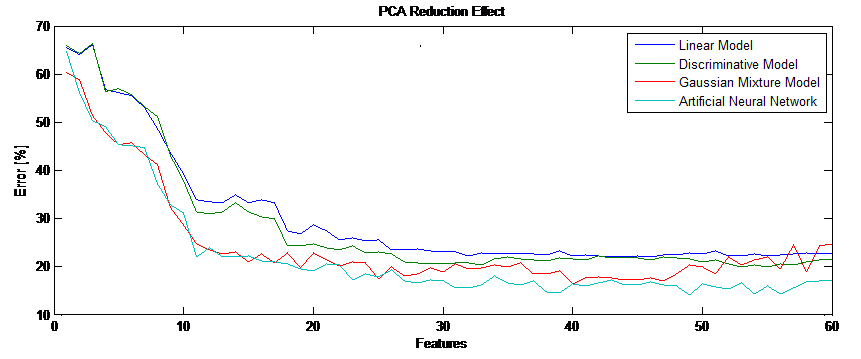
\includegraphics[scale=0.7]{billeder/PCAReductionEffect}
\caption{ Dimensions effect on Error }
\label{fig:DimError}
\end{figure}

%------------------------------------------------
